\documentclass[12pt, a4paper]{article}
\usepackage[utf8]{inputenc}

% Font
\usepackage{MinionPro}
\input glyphtounicode
\pdfgentounicode=1
\usepackage{microtype}
\usepackage[super]{nth}
\usepackage{csquotes}

% Format
\setlength{\parindent}{0.5in}
\setcounter{secnumdepth}{0}

% Language
\usepackage[american]{babel}

% Links
\usepackage[colorlinks=true, linkcolor=black, urlcolor=black, citecolor=black]{hyperref} 

% References
\usepackage[style=apa]{biblatex}
\DeclareSourcemap{
  \maps[datatype=bibtex]{
    \map{
      \pertype{book}
      \step[fieldset=location, null]
      \step[fieldset=address, null]
    }
    \map{
      \pertype{incollection}
      \step[fieldset=location, null]
      \step[fieldset=address, null]
    }
  }
}
\addbibresource{appendices.bib}
\renewcommand*{\bibfont}{\small}
% Figures
\usepackage{graphicx}
\usepackage[small, labelfont=it, labelsep=period]{caption}

% Tables
\usepackage{booktabs}
\usepackage{tabularx}
\usepackage{subcaption}

% Commands
\newcommand{\pest}[4]{$ \text{Pr} (\text{``us''} | \text{#1}) = #2$, $[#3, #4]$}
\newcommand{\pdif}[4]{$ \Delta\text{Pr} (\text{``us''} | \text{#1}) = #2$, $[#3, #4]$}

% Frontmatter
\title{\emph{Appendices for}\\Intergroup contact fosters\\more inclusive social identities}
\date{April 24, 2020}

\begin{document}

\maketitle

\section{Appendix A: Additional Measures}

We included additional measures to validate the triple crossed-categorization task and to replicate earlier research. We tested to what extent various social identity measures correlated with responses in the triple crossed-categorization task. We also assessed Karmic beliefs to replicate \citeauthor{cotterill_ideological_2014}'s (\citeyear{cotterill_ideological_2014}) finding that Karmic beliefs mediate the relationship between social dominance orientation and support for hierarchy-enhancing policies. We do not report results from this replication here, but make all data available online.

\subsection{Measures}

Group identification was measured with one item per ingroup \parencite{postmes_single-item_2013}: ``I identify with my [nationality/religion/caste group]'' ($1 = \textit{strongly disagree}$, $7 = \textit{strongly agree}$).

Social identity complexity \parencite{roccas_social_2002, schmid_antecedents_2009} was operationalized as the extent to which participants perceived their different group memberships as conceptually interrelated (\emph{similarity complexity}) and numerically overlapping (\emph{overlap complexity}). Two items measured similarity complexity for religion/nationality and for nationality/caste: ``How similar or different are the typical [Hindu/Indian] and the typical [Indian/person from your caste group] to each other?'' ($1 = \textit{very different}$, $5 = \textit{very similar}$, reverse coded), and ``Do you think that being [Hindu/Indian] means the same as being [Indian/from your caste group]?'' ($1 = \textit{means something very similar}$, $5 = \textit{means something very different}$).  Two items measured overlap complexity for religion/nationality: ``How many [Indians/ Hindus] do you think are [Hindus/Indian]?” (\%, $r = .63$). Three items measured overlap complexity for nationality and caste: ``How many Indians do you think are [GC, OBC, SC/ST]?'' (\%, $.33 \leq rs \leq .50$). Overlap items were reverse coded, so that higher scores indicated less perceived overlap.

\emph{Entitativity} \parencite{lickel_varieties_2000} was measured with six items: ``Being Indian is important to each Indian, no matter their caste or religion'', ``Indians of all castes and religions interact often with each other.'', ``Indians of all castes and religions are working towards shared goals'', ``What happens to one Indian also impacts other Indians'', ``Indians of all castes and religions depend on one another'', and ``Indians are similar to one another'' ($1 = \textit{strongly disagree}$, $7 = \textit{strongly agree}$, $\alpha = .80$). Participants were encouraged to ``take Indian/Indians to mean Indian citizens of all castes and religions'' when reading the items of this scale. This scale thus measured an inclusive conception of entitativity.

\emph{Karmic beliefs} \parencite{cotterill_ideological_2014} were measured with three items: ``my current caste group position reflects
my actions or deeds in my past life'', ``if I do good deeds in my current life they will positively influence my caste status in my future life'', and ``the caste group position I was born into reflects the Karma of my past life'' ($1 = \textit{strongly disagree}$, $7 = \textit{strongly agree}$).

\subsection{Correlates of categorization}

We explored how participants' responses in the triple crossed-categorization task related to other measures of social identification. To that end, we estimated the correlations between, on the one hand, the proportions of targets that participants had categorized as ``us'' in each of the six categories, and, on the other hand, the (aggregated) social identification variables described in the \emph{Measures} section. We derived the likelihood of the observed responses from a multivariate normal distribution: $$ \textbf{Y} \sim \text{MVNormal} (\mu , \textbf{S} ) $$ where $\textbf{Y}$ is the matrix of observed variable scores (columns) across participants (rows), $\mu$ is the vector of all variable means, and $\textbf{S}$ is the variance-covariance matrix across variables.

Figure~\ref{fig:a-1} shows the estimated correlations between participants' categorizations in the triple crossed-categorization task (from left to right) and various social identification variables (from top to bottom). Entitativity---the extent to which participants saw Indians of \emph{all} castes and religions as similar to one another, as depending on each other, as sharing a common fate, as working towards shared goals, and as valuing their shared identity---was positively correlated with the proportion of \emph{Indian, Hindu, GM} ($r = .16$, $[.04, .27]$, $\text{Pr} (r > 0|M) > .99$), \emph{Indian, Hindu, OBC} ($r = .21$, $[.09, .31]$, $\text{Pr} (r > 0| M) > .99$), \emph{Indian, Hindu, SC/ST} ($r = .10$, $[-.02, .22]$, $\text{Pr} (r > 0| M) = .97$), and \emph{Indian, Muslim, OBC} ($r = .18$, $[.07, .30]$, $\text{Pr} (r > 0| M) > .99$) targets participants categorized as ``us''.

\begin{figure}
\centering
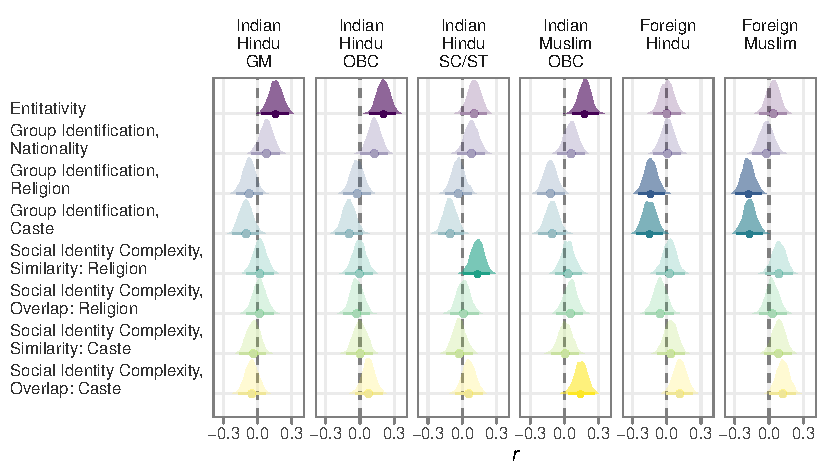
\includegraphics{../figures/appendices/appendices-e-1}
\caption[Correlations between social identity variables and target categorizations]{Correlations between various social identity variables (top to bottom) and the proportion of targets that participants had categorized as ``us'' in each target category (left to right). Points indicate the most likely estimate for a given correlation, while lines encompass the 97\% most likely estimates of that correlation. Curves show the density distributions of the posterior probabilities, based on all samples from the posterior probability distribution. Correlations for which $\text{Pr} (r > 0| M) > .99$ or $\text{Pr} (r < 0| M) > .99$ are shown in a darker shade.}
\label{fig:a-1}
\end{figure}

Group identification was only associated with participants' categorizations of foreign targets, not their categorizations of Indian targets. The extent to which participants identified with their religion was negatively correlated with how many \emph{foreign, Hindu} ($r = -.14$, $[-.25, -.02]$, $\text{Pr} (r > 0| M) > .99$) and \emph{foreign, Muslim} ($r = -.18$, $[-.29, -.07]$, $\text{Pr} (r > 0| M) > .99$) targets participant categorized as ``us''. I obtained similar correlations for the extent to which participants identified with their caste group, $r = -.15$, $[-.27, -.04]$, $\text{Pr} (r > 0| M) > .99$ and $r = -.17$, $[-.29, -.06]$, $\text{Pr} (r > 0| M) > .99$, respectively. The extent to which participants identified with their nationality was not associated with participants' categorizations---perhaps because there was a little variation in participants responses, with 81\% of participants strongly agreeing with the statement. Other variables were not systematically correlated with participants' responses in the crossed-categorization task (see Figure~\ref{fig:a-1}).

Correlations thus confirmed that participants' categorizations were more than a straight-forward reflection of the strength of their group identification, affirming the value of the crossed-categorization task for studying identification in contexts with multiple, cross-cutting group memberships. Furthermore, participants' perceptions of entitativity across caste and religions were associated with more inclusive construals of national identity, providing tentative evidence for its potential for fostering more inclusive identities.

\newpage

\section{Appendix B: Sample Size}

We ran simulations to determine the sample size required to obtain reasonably precise estimates of the model parameters of interest.\footnote{Bayesian data analysis does not usually allow for \textit{analytical} power analyses.} What made these simulations challenging is that multilevel models have more parameters than simple generalized linear models and that no clear default values exist to narrow down the parameter space for our simulations. We constrained our simulations in several ways:

\begin{enumerate}
\item We re-analysed existing data (kindly provided by \nptextcite{van_dommelen_construing_2015}) from a study of 91 Turkish Australians (46 women, 45 men) completing a version of the triple crossed-categorization task with eight target categories. We ran a model identical to Model~1 (Table~2, in the main text) which estimated participants' categorizations as varying across participants and across target categories. We could not estimate group differences across the participants' ingroup because all participants belonged to the same group.
\item We decided to focus our simulations on two kinds of parameters of interest. First, we considered how participants' categorizations of the eight target categories differed across three participant ingroups. Second, we considered how participants' categorizations varied as a function of a continuous predictor variable. As we could not estimate these parameters from the existing data, we used informative prior distribution to simulate plausible values for the corresponding model parameters.\footnote{We modeled differences between the three participant ingroups as $\beta_k \sim \text{Normal}(\beta_0, \sigma)$ with the prior distributions $\beta_0 \sim \text{Normal}(0, 1)$ and $\sigma \sim \text{Half-Student-t}(10, 0, 0.2)$, where $1 < k < 8$ was an index for the eight target categories. We modeled the fixed coefficient of the continuous predictor with the prior distribution $\beta_x \sim \text{Normal}(0, 1)$.}
\item We decided to run our simulations for samples of 3 (groups) x 100 (sample size per group) = 300 participants. This sample size reflects constraints in the number of potential participants available to us.
\end{enumerate}

\noindent First, we simulated 4,000 datasets of 300 participants by combining posterior predictive draws from the model fit to the existing data for the varying intercepts across participants and target categories, simulation draws from the informative prior distributions for the varying effects of participant ingroups and the fixed effect of the continuous predictor variable, and simulation draws from a $\text{Normal}(0, 1)$ distribution for values of the continuous predictor variables. Second, we randomly selected 10 of these datasets and estimated the relevant model parameters by applying a model akin to Model 4 (Table~2, in the main text).\footnote{We decided to use no more than ten samples as running these models was computationally expensive and as the precision of our estimates did not differ much across samples.} Third, we calculated the standard deviations of the posterior distributions (equivalent to standard errors in classical statistics) for all model parameters and all samples. 

Table~\ref{tab:b-1} shows the results of our simulations. For $N = 300$, our model estimated the (varying) effects of group differences with an average precision of $\textit{SD} = 0.41$ (0.34--0.50) and the (fixed) effect of a  continuous predictor with an average precision of $\textit{SD} = 0.17$ (0.14--0.21) on the log odds scale. As log odds are difficult to interpret, we translated these values to the change in the proportion of ``us'' categorizations that results from a +1\textit{SD} increase in log odds above the average log odds of ``us'' categorizations. We thus translate the average precision to $\Delta\Pr = .074$ for group differences and $\Delta\Pr = .033$ for the continuous predictor. As we expected group differences to be greater than individual differences in participants' categorizations, we concluded that 100 participants per group would yield reasonably precise estimates of the parameters of interest.

\begin{table}[!p]
\centering
\figureversion{lining, tabular}
\caption{Standard deviations of the posterior distributions for 17 parameters across 10 simulations. \textit{SD} is the average standard deviation across the 10 simulations while \textit{Min} is the minimum and \textit{Max} is the maximum. $\Delta\Pr$ is the change in the proportion of ``us'' categorizations for a +1\textit{SD} increase in log odds.}
\small	
\begin{tabular}{lrrrrr} \toprule
Parameter & $k$ & \textit{SD} & \textit{Min} & \textit{Max} & $\Delta\Pr$ \\
\midrule \addlinespace
  $\beta_\text{Group 1 - Group 2}$ & 1 & 0.42 & 0.33 & 0.51 & .076 \\
  $\beta_\text{Group 1 - Group 2}$ & 2 & 0.41 & 0.34 & 0.49 & .075 \\
  $\beta_\text{Group 1 - Group 2}$ & 3 & 0.40 & 0.33 & 0.48 & .073 \\
  $\beta_\text{Group 1 - Group 2}$ & 4 & 0.40 & 0.33 & 0.48 & .072 \\
  $\beta_\text{Group 1 - Group 2}$ & 5 & 0.40 & 0.32 & 0.46 & .072 \\
  $\beta_\text{Group 1 - Group 2}$ & 6 & 0.40 & 0.33 & 0.46 & .072 \\
  $\beta_\text{Group 1 - Group 2}$ & 7 & 0.40 & 0.33 & 0.47 & .073 \\
  $\beta_\text{Group 1 - Group 2}$ & 8 & 0.39 & 0.32 & 0.47 & .070 \\
  $\beta_\text{Group 1 - Group 3}$ & 1 & 0.43 & 0.35 & 0.52 & .077 \\
  $\beta_\text{Group 1 - Group 3}$ & 2 & 0.44 & 0.36 & 0.56 & .079 \\
  $\beta_\text{Group 1 - Group 3}$ & 3 & 0.42 & 0.35 & 0.53 & .076 \\
  $\beta_\text{Group 1 - Group 3}$ & 4 & 0.42 & 0.36 & 0.53 & .075 \\
  $\beta_\text{Group 1 - Group 3}$ & 5 & 0.42 & 0.35 & 0.54 & .075 \\
  $\beta_\text{Group 1 - Group 3}$ & 6 & 0.42 & 0.35 & 0.52 & .075 \\
  $\beta_\text{Group 1 - Group 3}$ & 7 & 0.42 & 0.36 & 0.52 & .075 \\
  $\beta_\text{Group 1 - Group 3}$ & 8 & 0.40 & 0.34 & 0.52 & .073 \\
	$\beta_x$                        &   & 0.17 & 0.14 & 0.21 & .033 \\
\addlinespace 
%\midrule $M$ & & 0.40 & 0.33 & 0.49 & .072 \\ 
\bottomrule
\end{tabular}
\label{tab:b-1}
\end{table}

\newpage

\section{Appendix C: Descriptive Statistics}

Table~\ref{tab:c-1} reports means and standard deviations for all variables. Tables~\ref{tab:c-2} to \ref{tab:c-5} report correlations between all variables for various ingroups and outgroups.

\begin{table}[!hp]
\centering
\figureversion{lining, tabular}
\caption{Means and standard deviations (in brackets) for all measured combinations of outgroups (rows) and ingroups (columns).}
\small	
\begin{tabular}{llrrr} \toprule
Variable & Outgroup & GM & OBC & SC/ST \\ \midrule \addlinespace
  Contact quantity & GM & - & 4.21 (0.96) & 3.84 (1.02) \\ 
  Contact quantity & OBC & 3.74 (1.12) & - & 4.04 (0.94) \\ 
  Contact quantity & SC/ST & 3.76 (1.10) & 3.92 (0.98) & - \\ 
  Contact quantity & Muslims & 3.49 (1.30) & 3.54 (1.17) & 3.49 (1.19) \\ \addlinespace
  Positive contact & GM & - & 4.03 (1.01) & 3.91 (1.05) \\ 
  Positive contact & OBC & 3.83 (1.01) & - & 3.84 (1.13) \\ 
  Positive contact & SC/ST & 3.68 (0.98) & 3.70 (1.19) & - \\ 
  Positive contact & Muslims & 3.40 (1.21) & 3.64 (1.13) & 3.53 (1.29) \\ \addlinespace
  Negative contact & GM & - & 2.17 (1.30) & 2.27 (1.30) \\ 
  Negative contact & OBC & 1.96 (1.19) & - & 2.38 (1.32) \\ 
  Negative contact & SC/ST & 1.99 (1.13) & 1.88 (1.13) & - \\ 
  Negative contact & Muslims & 2.44 (1.30) & 2.20 (1.20) & 2.28 (1.23) \\ \addlinespace
  Friendship & GM & - & 4.21 (0.84) & 3.95 (0.85) \\ 
  Friendship & OBC & 3.58 (1.00) & - & 4.03 (0.85) \\ 
  Friendship & SC/ST & 3.43 (0.96) & 3.66 (1.00) & - \\ 
  Friendship & Muslims & 3.20 (1.12) & 3.37 (0.95) & 3.30 (0.93) \\ \addlinespace
  (Dis-)advantage & GM & 2.83 (2.13) & 2.86 (2.02) & 4.08 (1.96) \\ 
  (Dis-)advantage & OBC & 4.89 (1.68) & 3.90 (1.81) & 4.11 (1.70) \\ 
  (Dis-)advantage & SC/ST & 5.44 (1.65) & 5.40 (1.79) & 4.30 (2.01) \\ 
  (Dis-)advantage & Muslims & 4.26 (1.83) & 4.34 (1.77) & 3.84 (1.96) \\ \addlinespace
  Policy support & OBC & 2.66 (1.35) & 3.79 (1.03) & 3.54 (0.94) \\ 
  Policy support & SC/ST & 1.91 (1.15) & 2.28 (1.18) & 4.22 (0.88) \\ 
  Policy support & Muslims & 2.62 (1.23) & 2.82 (1.17) & 3.28 (1.30) \\ \addlinespace
  Realistic threat & SC/ST & 3.79 (1.16) & 3.48 (1.06) & - \\ 
  Realistic threat & Muslims & 3.39 (1.09) & 3.06 (1.00) & 3.24 (1.10) \\ \addlinespace
  Symbolic threat & SC/ST & 3.28 (1.07) & 3.18 (1.06) & - \\ 
  Symbolic threat & Muslims & 3.60 (1.17) & 3.37 (1.12) & 3.53 (1.27) \\ \addlinespace
  SDO-D &  & 0.02 (0.71) & -0.04 (0.74) & 0.05 (0.78) \\ 
  SDO-E &  & 0.14 (0.72) & -0.06 (0.68) & -0.07 (0.82) \\  \bottomrule
\end{tabular}
\label{tab:c-1}
\end{table}


\begin{table}[!hp]
\centering
\figureversion{lining, tabular}
\caption{Correlations between variables for GM (above the diagonal) and SC/ST (below the diagonal) participants with people from other backward classes (OBCs) as the relevant outgroup.}
\small	
\begin{tabular}{rlrrrrrrrr} \toprule
\# & Variable & 1 & 2 & 3 & 4 & 5 & 6 & 7 & 8 \\ \midrule 
1 & Contact quantity &  &  .63 &  .01 &  .67 &  .22 & -.12 & -.06 & -.02 \\ 
  2 & Positive contact &  &  & -.12 &  .55 &  .04 &  .02 & -.08 & -.03 \\ 
  3 & Negative contact & -.28 &  &  &  .01 &  .01 &  .11 &  .13 &  .10 \\ 
  4 & Friendship &  .41 &  .49 &  &  &  .16 & -.06 & -.10 & -.06 \\ 
  5 & (Dis-)advantage &  .14 &  .12 & -.05 &  &  & -.22 & -.09 & -.03 \\ 
  6 & Policy support &  .11 &  .12 & -.19 &  .13 &  &  &  .14 &  .15 \\ 
  7 & SDO-D &  .11 &  .06 &  .15 &  .13 &  .14 &  &  &  .43 \\ 
  8 & SDO-E & -.05 &  .17 & -.03 &  .03 &  .14 &  .15 &  &  \\ 
\bottomrule
\end{tabular}
\label{tab:c-2}
\end{table}

\begin{table}[!hp]
\centering
\figureversion{lining, tabular}
\caption{Correlations between variables for OBC (above the diagonal) and SC/ST (below the diagonal) participants with people from general castes (GM) as the relevant outgroup.}
\small	
\begin{tabular}{rlrrrrrrr} \toprule
\# & Variable & 1 & 2 & 3 & 4 & 5 & 6 & 7  \\ \midrule 
1 & Contact quantity &  &  .64 & -.31 &  .60 & -.00 & -.10 & -.03 \\ 
  2 & Positive contact &  &  & -.27 &  .63 & -.12 & -.07 & -.11 \\ 
  3 & Negative contact & -.03 &  &  & -.27 & -.04 &  .00 & -.05 \\ 
  4 & Friendship &  .17 &  .42 &  &  & -.07 & -.08 & -.12 \\ 
  5 & (Dis-)advantage &  .06 & -.02 & -.04 &  &  &  .09 &  .01 \\ 
  6 & SDO-D &  .15 &  .08 &  .14 &  .14 &  &  &  .46 \\ 
  7 & SDO-E &  .06 & -.02 &  .15 & -.06 &  .10 &  &  \\  
\bottomrule
\end{tabular}
\label{tab:c-3}
\end{table}

\newpage

\begin{table}[!hp]
\centering
\figureversion{lining, tabular}
\caption{Correlations between variables for GM (above the diagonal) and OBC (below the diagonal) participants with Dalits (SC/ST) as the relevant outgroup.}
\small	
\begin{tabularx}{\linewidth}{r@{~~}X@{~~}rrrrrrrrrr} \toprule
\# & Variable & 1 & 2 & 3 & 4 & 5 & 6 & 7 & 8 & 9 & 10 \\ \midrule 
1 & Contact quantity &  &  .47 & -.14 &  .41 &  .28 & -.20 &  .25 &  .09 & -.03 & -.06 \\ 
  2 & Positive contact &  &  & -.30 &  .18 &  .31 &  .02 & -.08 & -.08 & -.03 & -.09 \\ 
  3 & Negative contact &  .05 &  &  & -.01 & -.15 &  .03 &  .16 &  .22 &  .13 & -.10 \\ 
  4 & Friendship &  .31 &  .40 &  &  &  .06 & -.10 &  .07 & -.05 & -.12 & -.10 \\ 
  5 & (Dis-)advantage & -.03 & -.02 & -.23 &  &  & -.21 &  .24 & -.06 &  .06 &  .14 \\ 
  6 & Policy support &  .13 &  .21 &  .12 & -.03 &  &  & -.33 &  .06 &  .30 &  .04 \\ 
  7 & Realistic threat &  .04 &  .10 &  .03 & -.03 &  .08 &  &  &  .39 & -.03 &  .02 \\ 
  8 & Symbolic threat & -.12 &  .02 &  .16 & -.08 & -.04 & -.05 &  &  &  .35 & -.03 \\ 
  9 & SDO-D & -.11 &  .01 &  .18 &  .09 &  .11 &  .07 &  .14 &  &  &  .43 \\ 
  10 & SDO-E & -.08 &  .11 &  .02 &  .04 &  .13 &  .15 &  .13 &  .10 &  &  \\ 
\bottomrule
\end{tabularx}
\label{tab:c-4}
\end{table}

\begin{table}[!hp]
\centering
\figureversion{lining, tabular}
\caption{Correlations between variables for all non-Muslims participants with Muslims as the relevant outgroup.}
\small	
\begin{tabularx}{\linewidth}{r@{~~}X@{~~}rrrrrrrrrr} \toprule
\# & Variable & 1 & 2 & 3 & 4 & 5 & 6 & 7 & 8 & 9 & 10 \\ \midrule 
1 & Contact quantity &  &  .64 & -.11 &  .61 &  .17 &  .10 & -.11 & -.18 & -.04 & -.01 \\ 
  2 & Positive contact &  .64 &  & -.18 &  .65 &  .14 &  .15 & -.19 & -.22 & -.04 & -.06 \\ 
  3 & Negative contact & -.11 & -.18 &  & -.12 & -.01 & -.08 &  .14 &  .22 &  .17 &  .02 \\ 
  4 & Friendship &  .61 &  .65 & -.12 &  &  .03 &  .11 & -.21 & -.25 &  .01 & -.03 \\ 
  5 & (Dis-)advantage &  .17 &  .14 & -.01 &  .03 &  & -.16 &  .11 &  .06 &  .02 &  .00 \\ 
  6 & Policy support &  .10 &  .15 & -.08 &  .11 & -.16 &  & -.17 & -.14 &  .05 & -.01 \\ 
  7 & Realistic threat & -.11 & -.19 &  .14 & -.21 &  .11 & -.17 &  &  .51 &  .10 &  .08 \\ 
  8 & Symbolic threat & -.18 & -.22 &  .22 & -.25 &  .06 & -.14 &  .51 &  &  .13 &  .07 \\ 
  9 & SDO-D & -.04 & -.04 &  .17 &  .01 &  .02 &  .05 &  .10 &  .13 &  &  .46 \\ 
  10 & SDO-E & -.01 & -.06 &  .02 & -.03 &  .00 & -.01 &  .08 &  .07 &  .46 &  \\ 
\bottomrule
\end{tabularx}
\label{tab:c-5}
\end{table}

\newpage

\section{Appendix D: Pilot Study}

Informed by local knowledge, we intended to rely on last names to unobtrusively communicate caste membership in the triple crossed-categorization task. To find the most prototypical stimuli, we compiled an initial set of 50 surnames, drawing on local knowledge, databases on naming preferences, and publicly available archives of Facebook usernames. We selected 10 surnames for each of five combinations of nationality, religion, and caste: (1) Indian Hindus of upper-caste backgrounds, (2) Indian Hindus of lower-caste backgrounds (Dalits), (3) Indian Muslims, (4) foreign Hindus, and (5) foreign Muslims. From these 50 names, we created 100 stimuli resembling identity cards, 50 with female first names and 50 with male first names. Each card had the target's first and last name, age (21--26 years), and religion (Hindu, Muslim) printed on them, as well as a flag corresponding to the target's nationality (Indian, Nepali, Sri Lankan, Bangladeshi) and a silhouette corresponding to the target's gender (adapted from \nptextcite{ma_chicago_2015}). Cards for female and male targets were identical in all attributes except first name and silhouette.

We asked 26 students (19 women, 7 men) of diverse caste groups (\emph{SC/ST}: 8, \emph{GM}: 10, \emph{OBC}: 8) and religious backgrounds (\emph{Hinduism}: 16, \emph{Islam}: 4, \emph{Christianity}: 5, \emph{Jainism}: 1) to review 25 of the 50 stimuli corresponding to their gender. For each stimulus, we asked participants which caste they thought the target most likely belonged to (\emph{SC/ST}, \emph{GM}, \emph{OBC}, \emph{GM or OBC}, \emph{Can't tell/Don't know}), how typical or unusual they considered the target's name for someone of that particular nationality, religion, and (if applicable) caste $(1 = \textit{very typical}, 6 = \textit{very unusual})$, and whether the target's name reminded them of anyone in particular (\emph{yes}, \emph{no}) and, if so, of whom. 

Participants' responses had important implications for designing the triple crossed-categorization task. On average, participants regarded all targets' names as at least ``somewhat typical'' $(1.42 \le \textit{Ms} \le 3.50)$. Names, however, were not enough to reliably cue caste membership---only $55\%$ to $83\%$ of participants identified even the most distinctive Dalit targets as Scheduled Caste~/ Scheduled Tribe (see Figure~\ref{fig:d-1}). Further, participants consistently categorized Muslim targets as Other Backward Class (see Figure~\ref{fig:d-2}), introducing a potential confound when comparing Muslim (OBC) and Hindu (GM) targets. Considering these findings, we decided to explicitly state caste membership (as reservation categories: GM, OBC, SC/ST) for Indian targets, and to add \emph{Indian, Hindu, OBC} targets as a sixth category.

\begin{figure}
\centering
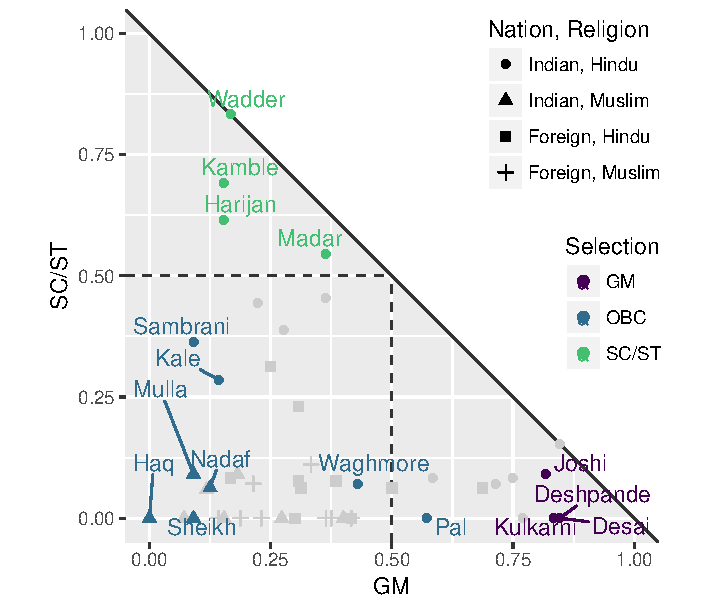
\includegraphics[scale=1]{../figures/appendices/appendices-a-1}
\caption[Proportion of SC/ST vs GM classifications per target stimulus (Pilot study)]{Proportion of SC/ST vs GM classifications per target stimulus. Targets in the upper-left quadrant were most often classified as SC/ST, while targets in the lower-right quadrant were most often classified as GM. Targets in the lower-left quadrant were more often classified as GM or OBC, or OBC than as SC/ST or GM, or could not be classified reliably. Colours highlight Indian targets selected as GM, OBC, and SC/ST stimuli, respectively, based on participants' categorizations in the pilot study. GM = General Merit, OBC = Other Backward Class, SC/ST = Scheduled Caste~/ Scheduled Tribe}
\label{fig:d-1}
\end{figure}

\begin{figure}
\centering
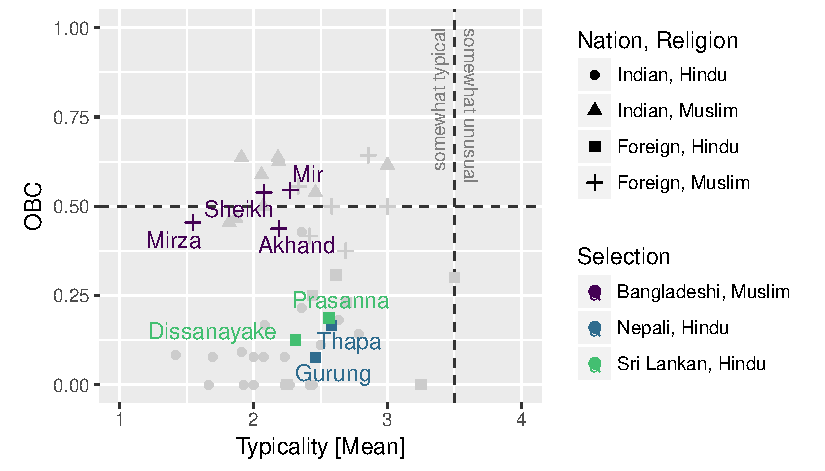
\includegraphics[scale=1]{../figures/appendices/appendices-a-2}
\caption[Foreign targets selected based on participants' average typicality ratings (Pilot study)]{Foreign targets selected as Sri Lankan, Hindu (2), Nepali, Hindu (2), and Bangladeshi, Muslim (4) stimuli, respectively, based on participants' average typicality ratings.}
\label{fig:d-2}
\end{figure}

For the final set of stimuli, we chose the four most prototypical targets for each of the six categories under study. We ranked Indian targets by the proportion of ``correct'' categorizations (e.g., $\Pr(\textit{OBC})$ for \emph{Muslim, OBC} targets) weighted by the inversed proportions of ``incorrect'' categorizations (e.g., $1 - \Pr(\textit{SCST})$ and $1 - \Pr(\textit{GM})$ for \emph{Muslim, OBC} targets). We selected the four highest-ranked (Category 1) \emph{Hindu, GM}, (2) \emph{Hindu, OBC}, (3) \emph{Hindu, SC/ST}, and (4) \emph{Muslim, OBC} targets (see Figure~\ref{fig:d-1}). We ranked foreign targets by their average typicality rating, and excluded targets who were categorized as General Merit or Scheduled Caste~/ Scheduled Tribe by $\ge 50\%$ of participants (to avoid obvious caste associations). We selected the two most typical (Category 5) \emph{Nepali, Hindu} and \emph{Sri Lankan, Hindu} targets, and the four most typical (6) \emph{Bangladeshi, Muslim} targets (see Figure~\ref{fig:d-2}). Based on the pilot study, we thus used $6~(\text{categories}) \times 4~(\text{targets}) = 24$ stimuli in the final study. Between $0\%$ and $44\%$ of participants ($\textit{Mdn} = 10\%$) recognised each selected name as familiar---in most cases, participants reported that targets reminded them of fellow students, former classmates, or co-workers.

\newpage

\section{Appendix E: Intergroup Threat}

We tested whether participants' perceptions of \emph{realistic} and \emph{symbolic threat} differed depending on the inclusiveness of their ingroup construals. Specifically, we examined whether participants reported feeling less threatened by Muslims and Dalits if they categorized more targets from these outgroups as ``us'' versus ``not us''. We excluded responses from Scheduled Caste/Scheduled Tribe participants to Scheduled Caste/Scheduled Tribe targets as we were interested in perceptions of \emph{inter}group threat. Models~0 to 7 estimated participants' mean responses, between $1 = \textit{strongly disagree}$ and $5 = \textit{strongly agree}$, to each of the $ 5 (\text{items}) \times 2 (\text{outgroups}) = 10$ items. Models derived the likelihood of the observed responses from the normal likelihood distribution: $$ y_{ij} \sim \text{Normal} (\mu_{ij}, \sigma) $$ where $y$ is the vector of participants' responses to each item, and $\mu_{ij}$ is the estimated mean response to item $i$ by participant $j$, $\sigma$ is the estimated residual variance (expressed as standard deviation).

Models~0 to 3 tested whether participants' responses differed across the two subscales (realistic vs symbolic threat) and across the two outgroups (Muslims vs Dalits).  Model 0 estimated item responses as varying between participants but fixed across all items: $$ \mu_{ij} = \beta_0 + \beta_{j} $$ where $\mu_{ij}$, the estimated mean response to item $i$ by participant $j$, equals $\beta_0$, the fixed intercept across items and participants, plus $\beta_j$, the varying intercept for participant $j$. Instead of assigning the same mean to all items, Model~1 included distinct intercepts for the two subscales: $$ \mu_{ij} = \beta_k + \beta_{j} $$ where $\beta_k$ is the fixed intercept for all items $i$ in subscale $k$, with $k = 1$ for realistic threat and $k = 2$ for symbolic threat. Model 2 instead estimated distinct intercepts for items concerning the two outgroups: $$ \mu_{ij} = \beta_l + \beta_{j} $$ where $\beta_l$ is the fixed intercept for all items $i$ for outgroup $l$, with $l = 1$ for Dalits and $l = 2$ for Muslims as the relevant outgroup. Model 3 tested the interaction of the two factors, and estimated distinct intercepts for all four combinations of subscales and outgroups: $$ \mu_{ij} = \beta_m + \beta_{j} $$ where $\beta_m$ is the fixed intercept for realistic threat from Dalits (when $m = 1$), for symbolic threat from Dalits (when $m = 2$), for realistic threat from Muslims (when $m = 3$), and for symbolic threat from Muslims (when $m = 4$). 

\begin{table}
\centering
\figureversion{lining, tabular}
\caption[Model comparison for intergroup threat]{Comparison of models estimating participants' intergroup threat.}
\small	
\begin{tabularx}{\linewidth}{r@{~}rXrrrrrr} \toprule
\# &  &  Description &  $R^2$ & $\textit{ELPD}$ & $\textit{SE}$ & $\Delta\textit{ELPD}$ & $\textit{SE}$ & $\frac{\Delta\textit{ELPD}}{\textit{SE}}$ \\ \midrule \addlinespace
0 &      & \textit{Varying intercept} & .31 & -3368.1 & 32.9 & - & - & - \\
1 & vs 0 & \textit{Subscales}         & .31 & -3368.9 & 32.9 & -0.8 & 0.6 & -1.3 \\
2 & vs 0 & \textit{Outgroups} & .32 & -3363.7 & 33.0 & 4.4 & 3.3 & 1.3 \\
3 & vs 0 & \textit{Subscales $\times$ Outgroups} & .33 & -3335.1 & 34.0 & 33.0 & 8.4 & 3.9  \\ \midrule
4 & vs 3 & \textit{Categorizations}   & .33 & -3335.5 & 34.0 & -0.3 & 0.6 & -0.5  \\
5 & vs 3 & \textit{Categorizations}   & .34 & -3330.5 & 34.0 & 4.7 & 3.6 & 1.3 \\
6 & vs 3 & \textit{Categorizations}   & .33 & -3336.7 & 34.0 & -1.5 & 0.7 & -2.1 \\
7 & vs 3 & \textit{Categorizations}   & .34 & -3332.8 & 34.0 & 2.3 & 3.6 & 0.6 \\ \addlinespace \bottomrule
\end{tabularx}
\label{tab:d-1}
\end{table}

Model~3, but not Models 1 and 2, improved upon the predictions of Model~0 (Table~\ref{tab:d-1}), showing that participants' perceptions of symbolic and realistic threat depended on whether the relevant outgroup was Muslims or Dalits. Specifically, participants reported more realistic ($ \beta_1 = 3.62$, $[3.49, 3.75]$) than symbolic ($\beta_2 = 3.21$, $[3.09, 3.33]$) threat from (same-religion) Dalits, $\text{Pr} (\beta_1 > \beta_2|M3) > .99$, but less realistic ($\beta_3 = 3.23$, $[3.06, 3.38]$) than symbolic ($\beta_4 = 3.47$, $[3.34, 3.61]$) threat from (different-religion) Muslims, $\text{Pr} (\beta_3 < \beta_4| M3) > .99$.

Models 4 to 7 tested whether the proportion of \emph{Indian, Muslim, OBC} and \emph{Indian, Hindu, SC/ST} targets participants had categorized as ``us'' was associated with less perceived threat from, respectively, Muslims and Dalits. Model~4 estimated this relationship as constant across outgroups and subscales: $$ \mu_{ij} = \beta_m + \beta_{j} + \beta_{Q1}x_{Q1,jl} $$ where $x_{Q1,jl}$ is the proportion [0--1] of targets belonging to outgroup $l$ that participant $j$ categorized as ``us'', and $\beta_{Q1}$ estimates the difference in threat perceptions between participants who categorized all four targets of outgroup $l$ as ``us'' and participants who categorized all targets of outgroup $l$ as ``not us''. Models~5 to 7 instead estimated distinct coefficients $\beta_{Q1,k}$ for each of the two subscales (M5), $\beta_{Q1,l}$ for each of the two outgroups (M6), or $\beta_{Q1,m}$ for each of the four combinations of subscales and outgroups (M7). Other than expected, Models~4 to 7 did not make better out-of-sample predictions than Model 3, indicating that whom participants considered ``us'' and ``not us'' was not associated with their perceptions of intergroup threat.

\newpage

\printbibliography

\end{document}